% Validity Ladder, Behavior Research Methods submission draft.
% Build: tectonic -X compile main.tex   (BibTeX runs automatically; apacite in natbibapa mode)
%
% Conventions used in the source (read before editing):
%   - One sentence per line.
%   - A line that carries a number ends with "% R: file.csv[; file.csv]" naming the receipt in
%     analysis/brm/ (or analysis_brm/*.md where noted). scripts/86_receipts.py parses these tags
%     into the receipts table (supplement S2) and checks each number against its file.
%   - \PATRICK{...} marks text only Patrick writes (gate rule 9: the claim, section points,
%     Discussion interpretations, conclusion). It prints as a red bracket so it cannot ship by accident.
%   - \CHECK{...} marks a fact still to confirm before submission.
\documentclass[man,12pt,floatsintext,natbib]{apa7}
\usepackage[natbibapa]{apacite}
\usepackage{amsmath,amssymb}
\usepackage{booktabs}
\usepackage{array}
\usepackage{graphicx}
\usepackage{xcolor}
\usepackage{catchfile}
% The abstract is read into a macro: apa7 cannot take \input inside \abstract.
\CatchFileDef{\abstracttext}{sections/00_abstract.tex}{}
\graphicspath{{figures/}}

\newcommand{\PATRICK}[1]{\textcolor{red}{\textbf{[PATRICK:} #1\textbf{]}}}
\newcommand{\CHECK}[1]{\textcolor{orange}{\textbf{[CHECK:} #1\textbf{]}}}
% Verdict words at level 2 are the rule's output; set them in small caps so they read as labels.
\newcommand{\vd}[1]{\textsc{#1}}
% Table notes as an environment (apa7's \tablenote is a one-argument command that needs threeparttable).
\newenvironment{tabnote}{\par\vspace{2pt}\small\raggedright}{\par}

\title{A Validity Ladder for LLM-Simulated Populations}
\shorttitle{Validity Ladder for Simulated Populations}
\authorsnames{Patrick Keough}
\authorsaffiliations{Independent researcher}
\leftheader{Keough}
\authornote{
  % ORCID: paste the real iD and uncomment the next line.
  % \addORCIDlink{Patrick Keough}{0000-0000-0000-0000}

  Data, code and every receipt file are at
  \url{https://github.com/pskeough/A-Validity-Ladder-for-LLM-Simulated-Clinical-Populations}.

  Correspondence concerning this article should be addressed to Patrick Keough, Email: pskeough@gmail.com
}

\abstract{\abstracttext}
\keywords{silicon samples, large language models, simulated participants, validity, measurement invariance, PHQ-8, NHANES}

\begin{document}
% apacite prints APA 6 "doi:" and "Retrieved from" forms; these give APA 7 output.
\renewcommand{\doiprefix}{https://doi.org/\ignorespaces}
\renewcommand{\BRetrievedFrom}{}
\maketitle

% Section 1. Introduction.

Behavioral researchers now prompt large language models (LLMs) with demographic personas and treat the answers as \emph{silicon samples}.
\citet{argyle2023outofone} used such samples to reproduce vote choice and opinion by group, \citet{park2024diminished} used them to replicate classic experiments, and \citet{lin2026simulators} describe their use in piloting instruments before fielding them.
For a study, a simulated sample costs little, reaches groups that are hard to recruit, and can be rerun whenever the design changes.
Each of these uses assumes that the simulated sample stands in for a real one in the respect the study measures.

In practice the stand-in assumption is checked unevenly.
Across eight social science journals, \citet{desai2026validating} found validation practice in LLM studies ``inconsistent and limited.''
\citet{park2024diminished} found GPT-3.5 answering with almost no variation where people vary, and \citet{bisbee2024synthetic} found synthetic opinion distributions narrower than the survey distributions they imitate.
\citet{lin2026workflow} proposed a workflow in which the validity a study needs rises with the claim it makes.
That workflow does not yet supply the tests themselves, each with a pass rule and a population reference, in an order a researcher can run on one model and report.

One persona from the corpus analysed here shows what reading individual answers misses.
Prompted as a single Black woman on Medicaid with a household income under \$35,000, GPT-4o-mini returns a PHQ-8 total of 8 on its first draw, a plausible answer in the mild band. % R: 85_worked_case.csv
Over thirty draws the same prompt averages 10.3. % R: 85_worked_case.csv
Adults in the National Health and Nutrition Examination Survey (NHANES) who share her race, sex, income and marital status average 4.7. % R: 85_worked_case.csv
None of her single answers would show that the simulated population she belongs to sits well above the real one.

We propose a protocol for the missing check, the validity ladder (Figure~\ref{fig:ladder}).
A gate first measures how many repeated draws make a persona's score precise enough to read.
Above the gate, level 1 tests whether a single draw is an answer pattern a person could give, and level 2 tests whether gaps between groups match the population's.
Level 3 tests whether the population level matches, and level 4 tests whether the items relate to one another as they do in people.
Each rung of the ladder, the gate or one of the levels, carries a statistic, a pass rule and the use a pass supports, and a simulated sample supports only the claims whose rungs it has passed.
With the rules frozen and released as code, a researcher can run the ladder on their own sample and report the verdicts.

The worked example applies the ladder to 28,800 PHQ-8 depression assessments from GPT-4o-mini, Gemini-3-Flash, DeepSeek-V3 and GLM-4.7, a corpus first collected for an earlier audit \citep{keough2026plausible} and rebuilt here from the raw answers. % R: corpus_v3_provenance.csv
A few repeated draws suffice to read each persona's mean, yet no model passes any level above the gate.
Single answers vary less than people's, and the models exaggerate the income gradient, place every group's level too high and distort the scale's structure.
Before these failures can be credited to the models, the ladder has to be shown not to fail real people.
Survey respondents drawn through the same design rarely fail any level, and failures planted at known sizes are caught by the level built to find them.

Three published silicon-sample datasets test whether the ladder travels beyond one instrument.
Feeling thermometers from \citet{bisbee2024synthetic}, vote choice and attitudes from \citet{argyle2023outofone} and opinion distributions from \citet{meister2025distributional} go through the same frozen rules.
The ladder keeps a few partisan gaps and leaves most other gaps failed, unresolved or unreadable, pointing toward narrower readings of each release's claims.

% Section 2. The ladder. Short rewrite of 2 Oct 2026, gated through mimesis voice=research,
% revised after Patrick's read (plain lead-in before each statistic; repository detail moved to
% the Open Practices Statement). Full specification: Supplement S7 and LADDER_SPEC.md.
% Level 2 reports three verdicts (kept, not kept, unresolved); the five regions name direction.

\section{The Validity Ladder}
\label{sec:ladder}

The ladder applies to any simulated sample in which a model answers a fixed instrument while conditioned on a persona.
One draw is one call to the model and the answer vector it returns.
A cell is one persona under one model and one prompt framing, and it holds $k$ draws whose mean score is the persona mean.
Figure~\ref{fig:ladder} summarises the gate and the four levels, with the question each asks, the statistic it reads and the use a pass supports.

The gate tests the base premise of any simulated sample, whether the model gives a persona a score consistent enough to read.
Each level above the gate supports a broader claim, moving from a single answer at level 1 to gaps between groups at level 2, the population's level at level 3 and the structure of the instrument at level 4.
A sample earns each claim separately, and the researcher reads off the claims their sample supports.
Without these checks, answers that look coherent are assumed coherent and a sample that looks typical is assumed free of bias.

A researcher deploys one model, so the ladder gives each model its own verdicts.
Pooling several models into one verdict can hide errors that run in opposite directions, as the sex gaps in Section~\ref{sec:results} show.
A pass means the test found no failure at the precision the data allow, and a level whose population reference is too imprecise to support any verdict records a stop in place of a pass or a fail.
The gate fixes $k$ for levels 2 and 3, and a failure at level 1 rules out single-draw uses only, so the other levels still run.
The rules and thresholds were fixed before any of the datasets in Section~\ref{sec:external} were analysed.
The thresholds are defaults that a user may change, and Supplement S7 gives the full specification, including estimators, bootstrap designs and multiplicity control.

\begin{figure}[tp]
% Figure 1 title (APA: number and title above the figure). The reading guide is fig1_ladder_note.tex.
% General map of the ladder, drawn by scripts/84d_fig1_ladder.py; no corpus or survey named.
\caption{The Validity Ladder}
\label{fig:ladder}

{\centering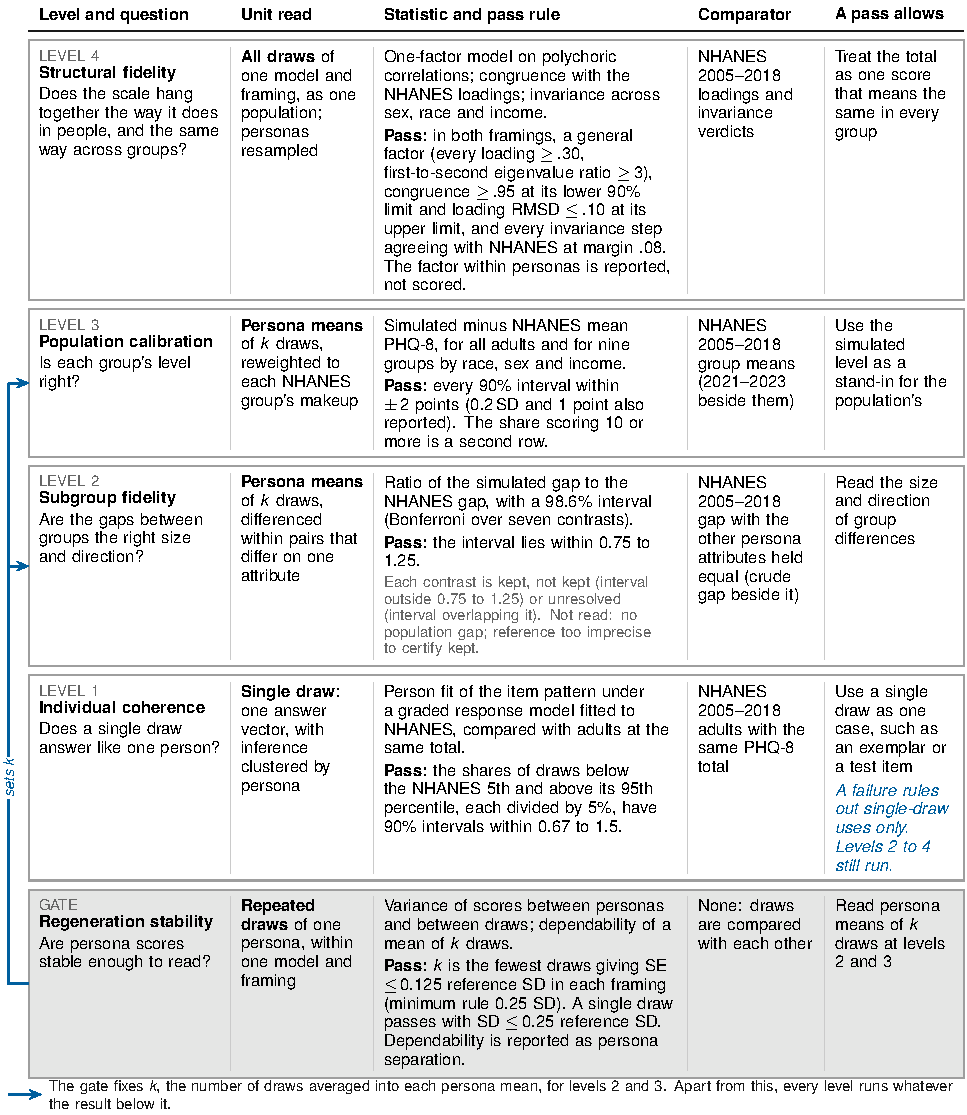
\includegraphics[width=\linewidth,height=0.71\textheight,keepaspectratio]{fig1_ladder.pdf}\par}
% Figure 1 note (below the figure).
\figurenote{Read from the gate at the bottom to level 4 at the top.
Each row gives the question a level asks, the unit it reads, its statistic and pass rule, what it is compared with, and the use a pass supports.
The gate sets $k$, the number of draws averaged into each persona mean, for levels 2 and 3.
A level-1 failure rules out single-draw uses only, so levels 2 to 4 run whatever level 1 finds.
Transgender and multiracial personas have no NHANES group of their own and never enter a group comparison.}

\end{figure}

\subsection{Gate: Regeneration Stability}
\label{sec:gate-method}

The gate asks how many draws must be averaged before a persona's score is precise enough to read.
Repeated draws of one persona differ because the model samples its answer, so each draw is the persona's own score plus draw-to-draw noise.
A generalizability study \citep{cronbach1972dependability,brennan2001gtheory} measures the two parts as variances, $\sigma^2_p$ for the spread of scores between personas and $\sigma^2_r$ for the spread of draws within one persona.
Averaging $k$ draws shrinks the noise in a persona mean, and its standard error and dependability are
\begin{equation}
\mathrm{SE}(k) = \sqrt{\sigma^2_r / k}, \qquad \phi(k) = \frac{\sigma^2_p}{\sigma^2_p + \sigma^2_r / k}.
\label{eq:phi}
\end{equation}
The standard error is the typical distance between a persona mean and the score the model would give over unlimited draws.
Dependability, from 0 to 1, is the share of the variation among persona means that reflects real differences between personas.

Persona means of $k$ draws may be read when $\mathrm{SE}(k)$ is at most 0.25 reference standard deviations in each framing, and the recommended $k$ brings it to 0.125 standard deviations.
On the PHQ-8 these tolerances are 0.98 and 0.49 points.
A single draw may be read as the persona's score only when the draw-to-draw standard deviation is itself at most 0.25 reference standard deviations.
Dependability is reported beside every verdict and required ($\phi \ge .80$) only for uses that compare or rank individual personas, because a faithful simulator inherits the population's small differences between cells.
Drawn through the persona design, real NHANES respondents reach a dependability of .70 at 30 draws. % R: analysis_brm/intermediate_panel/88_panel_verdicts.csv
A pass supports reading the persona mean of $k$ draws as the model's answer for that persona, and it says nothing about whether the answer is correct.

\subsection{Level 1: Individual Coherence}
\label{sec:l1-method}

Level 1 asks whether a single draw looks like an answer sheet a real person could give, and whether the draws are as varied as real people.
Real respondents with the same total score tend to endorse the common symptoms before the rare ones, and a minority answer in unusual patterns.
Person fit measures how typical an answer pattern is for its total.
A graded response model \citep{samejima1969graded} is fitted to the population reference with survey weights, and every respondent and every draw receives the standardised person-fit statistic $l_z^*$ \citep{drasgow1985appropriateness,snijders2001personfit,sinharay2016personfit}, which is low for an unusual pattern and high for an unusually regular one.
Each draw is then compared with real respondents who have the same total score.

The \emph{misfit ratio} is the share of a model's draws more unusual than 95\% of those respondents, divided by the 5\% expected, and the \emph{overfit ratio} is the share more regular than 95\% of them, divided by 5\%.
Both ratios equal 1 in a real population, and a ratio of 0.2 means the model gives a fifth as many such patterns as people do.
A model passes in a framing when the 90\% intervals of both ratios lie between $1/\tau$ and $\tau$.
The tolerance $\tau$ is the smallest of 1.5, 2 and 3 that covers how far every real subgroup by sex, race and ethnicity, income and survey cycle clearly departs from 1 when scored against the whole reference, with a floor of 1.5 set by the positive control (Section~\ref{sec:controls}).
On NHANES, $\tau = 1.5$. % R: l1_personfit_tolerance.csv
A model with too few patterns in both tails is called \emph{compressed}.
A pass supports using single draws as individual cases, such as exemplar vignettes or test items for a screener, and a compressed failure rules out uses that depend on the spread of real presentations.

\subsection{Level 2: Subgroup Fidelity}
\label{sec:l2-method}

Level 2 asks whether the gap between two groups, such as low- and high-income adults, has the population's size and direction.
The simulated gap $g$ compares personas that differ on one attribute and match on the rest, such as two personas identical except for income.
The population gap $\gamma$ is computed the same way in the survey, among people who match on the other attributes, and the crude survey gap is reported beside it.
The statistic is the ratio $\rho = g/\gamma$.
A ratio of 1 reproduces the population gap, 2 doubles it, 0 erases it, and a negative ratio reverses it.
Its interval is a Fieller interval, the standard interval for a ratio of two estimates \citep{fieller1954interval}, widened for the number of contrasts tested on each model, which gives 98.6\% intervals for seven contrasts.

A contrast is \vd{kept} when its whole interval lies between 0.75 and 1.25, \vd{not kept} when the interval lies wholly outside that range, and \vd{unresolved} when it overlaps it.
For a contrast that is not kept, the ratio gives the direction of the error, with ratios above 1.25 steepened, ratios from 0.25 to 0.75 attenuated, ratios near zero missing and negative ratios reversed.
Two stops are checked before any verdict.
A contrast is not read when the survey cannot tell its population gap from zero, and it is not read when the survey measures the gap too imprecisely for any simulated gap to be certified kept, unless the contrast is already clearly not kept.
A model passes level 2 when every contrast read is kept, fails when any is not kept, and is otherwise unresolved.
A pass supports reading the size and direction of group differences from the simulated sample, and it says nothing about either group's level.

\subsection{Level 3: Population Calibration}
\label{sec:l3-method}

Level 3 asks whether the simulated sample has a group's level, such as the mean PHQ-8 score of women or of low-income adults.
A persona grid is designed and not sampled, so before the comparison the personas are reweighted to the real mix of people in each group.
Each persona cell $c$ in a group $G$ is weighted by its share $p_c$ of the group in the reference, and the residual is
\begin{equation}
R_G = \sum_{c \in G} p_c\,(s_c - y_c),
\end{equation}
where $s_c$ is the persona mean and $y_c$ the mean of real respondents who match that persona \citep{holtsmith1979poststrat}.
A residual of $+2$ means the simulated group scores 2 points higher than the real group.
Its interval combines the draw error within cells with a design-based jackknife of the survey.

A row passes at tolerance $\delta$ when its 90\% interval lies inside $\pm\delta$, an equivalence test by two one-sided tests \citep{schuirmann1987tost,lakens2018tutorial}.
The researcher names $\delta$ as the smallest difference that matters for the use.
By default it is half a reference standard deviation, about 2 points on the PHQ-8, and 0.2 standard deviations is the strict alternative.
A model passes when every group row passes.
The share scoring at or above the instrument's cut point is a second row, because a correct mean can hide a wrong prevalence.
A pass supports using the simulated level as a stand-in for the group's level, within $\delta$, for the prompt, persona grid and survey period tested.

\subsection{Level 4: Structural Fidelity}
\label{sec:l4-method}

Level 4 asks whether the items of the instrument hang together as they do in people.
In real respondents the eight PHQ-8 items rise and fall together, so the total works as one depression score, and it works the same way in different groups.
All draws of one model in one framing are treated as one population, with personas as the resampling unit.
A one-factor model is fitted to the item correlations \citep{olsson1979polychoric} and checked against three rules.
R1 requires a general factor, one shared dimension behind the items, with every loading at least .30 and the first eigenvalue at least three times the second, or the reference's own value where the reference falls short.
R2 requires the items to load on that factor in the same pattern and with the same strength as in people, read as Tucker's congruence of at least .95 \citep{lorenzoseva2006congruence} and a root mean square difference in loadings of at most .10, each at the conservative end of its 90\% interval.
R4 requires the factor to work the same way across sex, race and income wherever it does in people, read on the RMSEA of each invariance step \citep{savalei2024rmsea} against a margin of .08.

A model passes level 4 when it passes all three rules in every framing.
Passing R1 and R2 supports scoring the total as one score with item weights like people's.
Passing R4 adds that a group comparison of the total means the same in the simulation as in people, so passes at levels 2 and 3 are read beside it.
A diagnostic (R3) also reports whether the factor holds among draws of one persona, as it does among people who share a demographic profile.

% Section 3. Worked example: data. Short rewrite of 2 Oct 2026. Generation details, resend
% provenance and the control-run designs are in Supplement S1 and S3; the pre-rewrite text is in
% _pre_rewrite_2026-10-02/sections/03_data.tex.

\section{Worked Example}
\label{sec:data}

\subsection{Data}

The worked example uses the corpus of \citet{keough2026plausible}, in which language models answered the eight-item Patient Health Questionnaire depression scale (PHQ-8; \citealp{kroenke2009phq8}) as demographic personas.
Four models, GPT-4o-mini, Gemini-3-Flash, DeepSeek-V3 and GLM-4.7, generated the corpus through OpenRouter between 28 December 2025 and 11 January 2026. % R: corpus_v3_provenance.csv
The persona grid crosses race (Asian, Black, Hispanic, multiracial, White), gender identity (cisgender and transgender women and men), income (three levels) and relationship status (married, single), for 120 personas.
Income was stated as a dollar-and-insurance label, from ``Low (<\$35k, Medicaid)'' to ``High (>\$250k, Concierge)''.
Each persona answered 30 times under each of two framings, one listing its attributes as fields (clinical) and one giving them as a first-person self-description (narrative).
A shared system prompt cast the model as a ``Clinical Simulation Engine'' answering from ``the statistical likelihood of symptoms for this specific demographic intersection in the US population''.
No sampling parameter was set, so every draw ran at the provider's default decoding.
The corpus holds 28,800 assessments, of which 28,799 have a valid PHQ-8. % R: corpus_v3_provenance.csv; l1_personfit_main.csv
Calls lost to API outages were resent in January under the same prompt, and every rung gives the same per-model verdicts without them (Supplement S3).
Supplement S1 prints the prompts, and the generation code is released with the data.

The population reference is the 36,274 adults in NHANES 2005--2018 who answered all eight PHQ-8 items, analysed with the survey's weights and design \citep{johnson2013nhanes,chen2018nhanes,nchs2018analytic}. % R: l1_nhanes_sample_flow.csv; analysis_brm/L4.md
Income is the ratio of family income to the poverty line, banded below 1.3, from 1.3 to 3.5, and above 3.5, and each persona's income label is mapped to one band.
Forty-eight of the 120 personas have a matching group in the survey.
NHANES records sex and not gender identity, and it does not identify multiracial adults on their own, so transgender and multiracial personas enter levels 1 and 4, which read the whole simulated population, and no group comparison.
NHANES 2021--2023 and other reference choices are sensitivity analyses in Supplement S3.

% Section 3.2. Worked example: results.

\subsection{Results}
\label{sec:results}

\begin{table}[!ht]
\centering
\caption{Ladder Verdicts per Model in the Worked Example}
\label{tab:verdicts}
\small
\newcolumntype{P}[1]{>{\raggedright\arraybackslash}p{#1}}
\begin{tabular}{@{}lP{2.1cm}P{2.3cm}P{1.9cm}P{1.9cm}P{2.5cm}@{}}
\toprule
Model & Gate: draws needed (min.\ / rec.) & Level 1: single draws & Level 2: income gap ratio & Level 3: overall residual & Level 4: structure \\
\midrule
DeepSeek-V3 & Pass (3 / 9) & Fail, compressed & Fail, 1.91 & Fail, +4.6 & Fail, no general factor \\ % R: gate_dstudy.csv; l2_headline.csv; 80d_headline.csv
Gemini-3-Flash & Pass (3 / 10) & Fail, compressed & Fail, 5.07 & Fail, +2.6 & Fail, loadings (R2) and invariance (R4) \\ % R: gate_dstudy.csv; l2_headline.csv; 80d_headline.csv
GPT-4o-mini & Pass (4 / 13) & Fail, compressed & Fail, 2.16 & Fail, +4.7 & Fail, no general factor \\ % R: gate_dstudy.csv; l2_headline.csv; 80d_headline.csv
GLM-4.7 & Pass (6 / 21) & Fail, too few atypical & Fail, 5.03 & Fail, +2.1 & Fail, loadings (R2) and invariance (R4) \\ % R: gate_dstudy.csv; l2_headline.csv; 80d_headline.csv
\bottomrule
\end{tabular}
\vspace{4pt}
\begin{tabnote}
\textit{Note.} Gate: draws needed for a persona mean's standard error to reach 0.25 (minimum) and 0.125 (recommended) NHANES standard deviations, the larger of the two framings. Level 2: ratio of the simulated to the standardised NHANES gap between low- and high-income personas, where 1 reproduces the gap. Level 3: post-stratified simulated minus NHANES mean PHQ-8, in points. Level 4: R2, loadings stronger than people's; R4, the factor differs across income where it does not in NHANES. Full per-level tables are in Supplement S4.
\end{tabnote}
\end{table}
\FloatBarrier

Table~\ref{tab:verdicts} gives every model's verdict at each rung, and Figure~\ref{fig:panels} shows what each failure looks like.
All four models pass the gate and fail every level above it.

\begin{figure}[tp]
% Figure 2 title. Drawn by scripts/84e_fig2_ladder_panels.py from analysis/brm/gate_dstudy.csv,
% l1_summary.csv, 80d_headline.csv and l4_structure.csv. Every level-2 interval is in Supplement Figure S1.
\caption{What Each Failure Looks Like in the Worked Example}
\label{fig:panels}

{\centering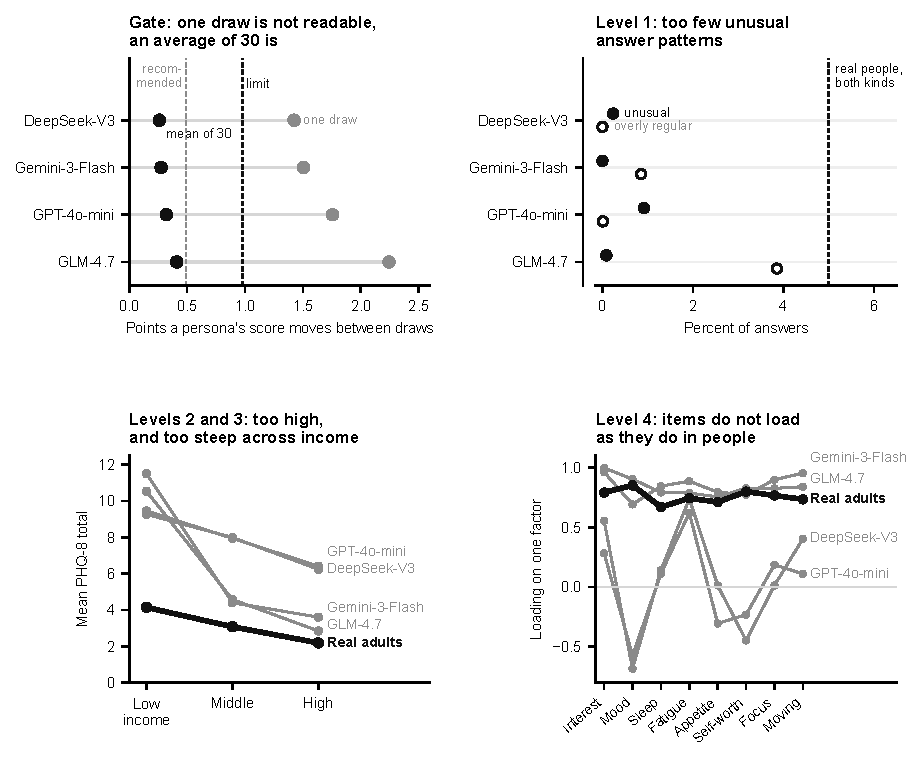
\includegraphics[width=\linewidth]{fig2_ladder_panels.pdf}\par}
% Figure 2 note (below the figure): how to read each panel.
\figurenote{Gate: how far a persona's PHQ-8 total moves between draws, for one draw (the draw standard deviation, larger framing) and for the mean of 30 (its standard error), against the gate's limit of 0.98 points and recommended level of 0.49. % R: gate_dstudy.csv
Level 1: percent of draws more unusual (filled) or more regular (open) than 95\% of NHANES adults with the same total, both framings, where real people give 5\% of each.
Levels 2 and 3: post-stratified mean PHQ-8 total in each income band.
Level 4: loading of each PHQ-8 item on a single factor in the narrative framing. DeepSeek-V3 and GPT-4o-mini have no general factor, and Gemini-3-Flash and GLM-4.7 follow the human pattern with loadings stronger than people's.
Every level-2 interval is in Supplement Figure S1.}

\end{figure}

\paragraph{Gate.}
No model can be read from a single draw.
The draw-to-draw standard deviation is 1.25 to 2.24 points in every model and framing, above the 0.98-point tolerance. % R: gate_dstudy.csv
Averages of 30 draws pass in every model, and the minimum rule needs 3 to 6 draws. % R: gate_dstudy.csv
Two draws of one persona fall in different PHQ-8 severity bands 35.2\% of the time [33.6, 36.8]. % R: gate_bandflip_summary.csv
In a separate decoding control on 12 personas, setting GPT-4o-mini's temperature to 0 cut its draw variance to 12.5\% of the default without separating personas any better (Supplement S1.10). % R: gate_decoding_link.csv
Every reading that follows therefore uses averaged draws.

\paragraph{Level 1.}
No model passes level 1, in either framing or at any tolerance up to 3. % R: l1_personfit_verdicts_tau.csv
At matched totals NHANES puts 5\% of adults in each tail of person fit, and the models put 0.0\% to 1.0\% in the unusual tail and 0.0\% to 4.3\% in the regular tail. % R: l1_summary.csv
Three models are compressed, and GLM-4.7 is short of unusual patterns alone.
The models also weight depressed mood more heavily than people do, scoring 0.16 to 0.51 points higher at matched totals on depressed mood and 0.22 to 1.11 points lower on fatigue, one of the physical symptoms people report first. % R: l1_personfit_item_profile.csv
They reuse answer sheets as well, giving two different personas the identical answer vector 4.6 to 39 times as often as two NHANES adults with the same total. % R: l1_pattern_reuse.csv
Any use that treats a draw as a person, from a vignette bank to a test set for a screener, would draw from a pool missing almost all of the unusual presentations that one in twenty real respondents give.

\paragraph{Level 2.}
Every model fails level 2 on income, and Supplement Figure S1 gives every interval.
The gap between low- and high-income personas is 1.91 (DeepSeek-V3) to 5.07 (Gemini-3-Flash) times the population gap. % R: l2_headline.csv
Of the 12 per-model income contrasts, 10 are steepened, and the survey measures the other two gaps too imprecisely to certify kept. % R: l2_headline.csv; l2_verdicts.csv
We read the size of the low-to-high ratio as partly a product of how the persona's income label is matched to the survey. % R: l2_verdicts.csv
Matching on the dollar amount in the label (Supplement S3) brings the ratio down to 1.04 for DeepSeek-V3 and 1.18 for GPT-4o-mini, which leaves both contrasts unresolved, and Gemini-3-Flash and GLM-4.7 stay steepened at 2.76 and 2.74. % R: l2_verdicts.csv
Under that matching DeepSeek-V3 and GPT-4o-mini still steepen the middle-to-high gap (3.29 and 2.89), leaving every model failing level 2. % R: l2_verdicts.csv
On the sex gap the models disagree, with GPT-4o-mini and DeepSeek-V3 reproducing a quarter to two fifths of it (ratios 0.23 and 0.41), GLM-4.7 doubling it (2.06) and Gemini-3-Flash unresolved. % R: l2_headline.csv
Pooled over the four models the ratio is 0.97, a near match built from errors in opposite directions. % R: l2_headline.csv
No racial contrast is kept in any model.
Among adults matched on income, sex and marital status, the survey cannot tell the Hispanic--White gap from zero and measures the Black--White gap too imprecisely to certify kept, and GPT-4o-mini's Black--White gap is still not kept. % R: l2_stop.csv; l2_headline.csv
For a researcher, these verdicts rule out estimating from any of these samples how depression differs by income, sex or race.
Because the survey measures the Black--White and Hispanic--White gaps too imprecisely to certify any simulator, a study of those gaps needs a larger or more targeted reference before the ladder can read it.

\paragraph{Level 3.}
Every simulated population is more depressed than NHANES.
After reweighting, the overall residual is +2.1 points for GLM-4.7, +2.6 for Gemini-3-Flash, +4.6 for DeepSeek-V3 and +4.7 for GPT-4o-mini. % R: 80d_headline.csv
All 40 model-by-group residuals are positive, and no model passes all ten groups at 2 points. % R: 80d_pass_counts.csv; 80d_model_verdicts.csv
In every model the largest residual is in the low-income band. % R: 80c_l3_results.csv
The failure holds under all eight reference specifications, including NHANES 2021--2023, and only whether the national row passes depends on the reference chosen (Supplement S3). % R: 89_l3_spec_range.csv; 89_l3_spec_range_summary.csv
Prevalence, the share scoring 10 or more, errs in a different pattern from the mean.
In the low-income band 55.5\% of simulated respondents score 10 or more, against 13.6\% of real adults. % R: 80d_headline.csv
Across the middle and high bands the simulated share is too low although the mean is too high, and DeepSeek-V3's overall prevalence looks correct only because its low-income excess cancels these shortfalls. % R: 80d_headline.csv; 80d_model_verdicts.csv
Read as a stand-in for a survey, these samples would overstate depression for every group, most of all among low-income adults.

\paragraph{Level 4.}
No model passes level 4.
DeepSeek-V3 and GPT-4o-mini have no general factor, with first-to-second eigenvalue ratios of 1.09 to 1.73 against 7.47 in NHANES. % R: l4_structure.csv
Gemini-3-Flash and GLM-4.7 have a factor with the human pattern of loadings (congruence .990 to .998), and the loadings are stronger than people's. % R: l4_structure.csv
Gemini-3-Flash fails R2 in both framings and GLM-4.7 in the narrative framing, and both fail invariance across income, which holds in NHANES. % R: l4_r2_size.csv; l4_invariance.csv
In these two models 48\% to 64\% of item variance lies between personas, against 3.5\% between demographic cells in NHANES, and draws of one persona share no general factor. % R: l4_between_within.csv
Built from differences between persona means, their factor rests on the same uniformity within personas that level 1 found.
For a researcher, the PHQ-8 total from DeepSeek-V3 or GPT-4o-mini cannot be scored as a single measure, and in Gemini-3-Flash and GLM-4.7 a comparison of the total across income levels lacks the meaning it carries in NHANES.

\paragraph{One persona.}
Followed through the ladder, the introduction's persona carries each verdict on a single case.
She is a single Black woman on Medicaid with an income under \$35,000, and GPT-4o-mini gives her 30 clinical draws ranging from 7 to 16. % R: 85_worked_case.csv
Her first draw of 8 lands in the mild band and her mean of 10.3 in the moderate band, so her readable score is the average. % R: 85_worked_case.csv
Her 60 draws are each plausible as human answers and together less varied than real people at her severity, repeating the level 1 failure. % R: 85_worked_case.csv
Her mean over both framings, 10.0, exceeds the 4.7 of matched NHANES adults by 5.3 points, repeating the level 3 excess. % R: 85_worked_case.csv
Level 2 reaches her only through the gaps her groups form with others.

\begin{table}[!ht]
\centering
\caption{Claims a Study Might Make From This Corpus, and What the Ladder Allows}
\label{tab:claims}
\small
\newcolumntype{P}[1]{>{\raggedright\arraybackslash}p{#1}}
\begin{tabular}{@{}P{1.4cm}P{5.5cm}P{7.4cm}@{}}
\toprule
Rung & Claim & On this corpus \\
\midrule
Gate & A persona's score can be read from one response. & \textbf{No.} Two draws of one persona fall in different severity bands 35.2\% of the time. \\ % R: gate_bandflip_summary.csv
Gate & The average of 30 responses is the model's score for that persona. & \textbf{Yes,} for all four models, which need 3 to 6 draws under the minimum rule. \\ % R: gate_dstudy.csv
Level 1 & A single response can stand in for a real patient. & \textbf{No.} Unusual answer patterns are 0.0\% to 1.0\% of draws, against 5\% of people. \\ % R: l1_summary.csv
Level 2 & Low-income adults score higher than high-income adults, by this much. & \textbf{Direction only.} The gap is 1.91 to 5.07 times its size in the population. \\ % R: l2_headline.csv
Level 2 & Women score higher than men, by this much. & \textbf{No.} Two models shrink the gap, one doubles it and one is unresolved. \\ % R: l2_headline.csv
Level 2 & Black and White adults differ by this much. & \textbf{Not certifiable.} The survey measures this gap too imprecisely to certify any model. \\ % R: l2_stop.csv
Level 3 & This share of low-income adults is depressed. & \textbf{No.} 55.5\% of low-income simulated respondents score 10 or more, against 13.6\% of real adults. \\ % R: 80d_headline.csv
Level 3 & Depression in the population is this high overall. & \textbf{No.} Every model is 2.1 to 4.7 points too high overall. \\ % R: 80d_headline.csv
Level 4 & The PHQ-8 total is one score that means the same in every group. & \textbf{No.} Two models have no general factor, and in the other two the factor differs across income. \\ % R: l4_structure.csv; l4_invariance.csv
\bottomrule
\end{tabular}
\end{table}

\paragraph{Summary.}
Read one at a time, every model's answers look like believable patients, and averages of a few draws are stable enough to read.
A researcher who checked this sample by reading its answers, or by the stability of its scores, would have accepted it.
Above that stable score the ladder fails the same sample on every use, finding its individual answers too uniform, its income gradient exaggerated, every group too depressed and its scale total without the structure the PHQ-8 has in people.

\paragraph{What this example does not show.}
These verdicts describe four base models under one prompt family, with one wording per attribute, one persona per demographic cell, no age in the personas and the PHQ-8 items in a fixed order.
The shared system prompt asked for the statistical likelihood of symptoms for each persona.
Removing that instruction did not remove the excess at level 3.
When a prompt control on 12 personas (Supplement S1.9) asked each model to answer as the person described, DeepSeek-V3 and GPT-4o-mini scored 5.8 to 7.4 points above NHANES in every income band, compared with 4.0 to 5.3 under the corpus prompt, while Gemini-3-Flash's low-income excess grew from 8.9 to 10.0 points. % R: ../prompt_control_results.csv
Each income label also paired a dollar amount with an insurance type, a cue the prompt control left unchanged.
Transgender and multiracial personas have no NHANES comparison group and were not tested at levels 2 and 3.
A different prompt, a persona grounded in real respondents or a fine-tuned simulator could pass where these models fail, and running the ladder on that sample would show whether it does.

% Section 5. Controls. Source: analysis_brm/CONTROLS.md (scripts 83a-83g), decision 15.
% Note: the 200-replicate positive control scores level 4 on R1, R2 and R3. R4 is read in the
% intermediate panel (scripts 88, 88b, 88c; 70 replicates, R4 on 25), and the text says which is which.

\section{Controls: Real People and Planted Failures}
\label{sec:controls}

Every model fails every rung above the gate, so the rungs have to be shown to pass real people and to detect failures of a known size.

\paragraph{Design.}
Each replicate splits the NHANES 2005--2018 adults at random into two halves, stratified by the 48 persona cells.
One half supplies respondents and the other half is the reference.
A pseudo-model has the corpus design: 120 personas, two framings and 30 draws.
Each draw is a respondent from the donor half, drawn within the persona's cell with probability proportional to the examination weight, and it keeps that respondent's eight item scores.
Transgender and multiracial personas draw from the closest available group and, as in the main analysis, enter levels 1 and 4 only.
Four independent pseudo-models form a panel, and there are 200 replicates. % R: analysis_brm/CONTROLS.md
Planted failures are applied to the same panels at a grid of doses: shuffling a draw's item values (incoherence), replacing a draw with the most typical vector at its total (compression), scaling a group gap by a factor $g$, shifting every persona mean by $d$ points, and rebuilding draws item by item from other draws of the same persona (removing within-persona covariance).
Each rung is read with its own rule.
Run on the real corpus with the full reference, the control code reproduces every published rung number, 303 of 303 checks. % R: 83a_receipt.csv

\paragraph{What real people pass.}
The level-1 rule is read per framing, and under it real respondents pass both framings in 92.9\% of 70 replicates, with the remaining replicates unresolved and none failed. % R: analysis_brm/intermediate_panel/88_confusion.csv
The pseudo-model passes level 3 on all ten groups in 100\% of replicates at 2 points and 98.1\% at 1 point. % R: 83c_l3.csv
It holds R1 and the R3 diagnostic in both framings in all 200 replicates, and R2 in all 40 replicates of the R2 calibration (loading RMSD upper limit .044 on average). % R: 83c_l4.csv; 83h_r2_size.csv
Real respondents are unresolved on R4 at the .08 margin in 24 of 25 replicates and fail it in 1, since 24 to 40 personas per group leave some invariance steps unresolved. % R: analysis_brm/intermediate_panel/88_confusion.csv; analysis_brm/intermediate_panel/88_r4_steps.csv
Making three items independent within the low-income group produces an R4 failure in 25 of 25 replicates, located at the income metric step. % R: analysis_brm/intermediate_panel/88_confusion.csv; analysis_brm/intermediate_panel/88_r4_steps.csv
At level 2, a determinate wrong verdict occurs in at most 1.0\% of readings at any dose and scope. % R: 83c_l2.csv
The level-2 intervals cover the true ratio in .986 to 1.000 of replicates per model, against .986 nominal. % R: 83c_l2_coverage.csv

\paragraph{Planted failures are detected.}
Table~\ref{tab:controls} gives, for each rung, the dose at which a planted failure is detected in at least 95\% of replicates, beside the distortion the real models show.
At levels 3 and 4 and for compression at level 1, the real distortion lies beyond the detected dose.
At level 2 the control's reference is a half sample, with twice the variance of the full survey, and per-model detection needs a threefold gap. % R: 83c_l2.csv
Two models' real income ratios (1.9 and 2.2) lie below that dose, and against the full reference the rung still names both \vd{steepened}. % R: l2_headline.csv

\begin{table}[tp]
\centering
\caption{Detection of Planted Failures, Against the Distortions the Models Show}
\label{tab:controls}
\small
\setlength{\tabcolsep}{4pt}
\begin{tabular}{@{}l>{\raggedright\arraybackslash}p{4.1cm}>{\raggedright\arraybackslash}p{3.9cm}>{\raggedright\arraybackslash}p{4.4cm}@{}}
\toprule
Rung & Planted failure & Detected in $\ge$95\% from & Real models \\
\midrule
Level 1 & Share of draws with item values shuffled & 40\% of draws & Not seen \\
Level 1 & Share of draws replaced by the most typical vector at the same total & 80\% of draws & Misfit ratio 0.00 to 0.18 (both framings); a 100\% dose reaches 0.33 \\
Level 2 & Income or sex gap scaled by $g$ & $g = 3$ per model (97.4\% to 100\%) & Low minus High, standardised: 1.9 to 5.1 per model \\
Level 3 & Every persona mean shifted by $d$ points & $d = 2$ at the 2-point tolerance (100\%) & $+2.1$ to $+4.7$ points overall \\
Level 4 & Share of draws decorrelated within persona & 50\% fails R2 in 100\%; 75\% fails R1 in 98.5\% & Within-persona $\lambda_1/\lambda_2$ 1.23 to 1.59, reached by the planted dose between 75\% (1.71) and 100\% (1.03) \\
\bottomrule
\end{tabular}
\vspace{4pt}
\begin{tabnote}
\textit{Note.} 200 replicates of a four-model panel of NHANES pseudo-models. Doses are nested, so a draw altered at one dose is altered at every larger dose. Per-dose detection rates for every rung and tolerance are in Supplement S5. % R: 83c_l1.csv; 83c_l2.csv; 83c_l3.csv; 83c_l4.csv; 83h_r2_size.csv; analysis_brm/L1.md
\end{tabnote}
\end{table}

\paragraph{What level 2 can and cannot certify.}
At NHANES precision, level 2 can detect distortion and cannot certify faithfulness.
In a simulation at the corpus's own precision, a faithful model is named \vd{kept} alone in at most 37\% of readings for the low-to-high income gap and 20\% for the sex gap, and in under 1\% for every other contrast. % R: 83f_l2_parametric_power.csv
These are the most favourable settings, the draw-only standard error at the most precise model, and under the primary pairs standard error neither rate exceeds 2\%. % R: 83f_l2_parametric_power.csv
For the sex and low-to-high income gaps, a faithful model usually receives a two-region verdict that contains \vd{kept}; for the other five contrasts the population gap is too imprecise to certify \vd{kept}, and the rung records that stop. % R: 83f_l2_parametric_power.csv
A twofold steepening of an income or sex gap is named correctly in 87\% to 100\% of draws under the draw-only standard error. % R: 83f_l2_parametric_power.csv
At the audit's own precision, the Black--White and Hispanic--White contrasts of a faithful model are stopped in 99.9\% of per-model readings. % R: 83c_l2.csv
The same design returns these stops for a faithful model, so the stops on race in the Results come from the reference and not from the models.

\paragraph{Intermediate simulators.}
Table~\ref{tab:panel} reads seven simulator types, all built from NHANES respondents through the corpus design, at every rung over 70 replicates. % R: analysis_brm/intermediate_panel/88_confusion.csv
Real respondents pass the gate and level 3 in every reading, level 1 in 92.9\% of replicates, and R1 and R2 in every replicate, and level 2 fails them in no reading. % R: analysis_brm/intermediate_panel/88_confusion.csv
Each planted failure trips the rung it targets. % R: analysis_brm/intermediate_panel/88_confusion.csv
Independent items fail level 1, R1 and R2 in every replicate, shifted samples fail level 3 in every reading, compressed samples fail level 1 in every replicate, non-invariant samples fail R4 in all 25 replicates, and a doubled income gap fails level 2 in 92.5\% of per-model readings. % R: analysis_brm/intermediate_panel/88_confusion.csv
The doubled gap also fails level 3 in 14.6\% of readings, because raising the low-income personas raises that group's level. % R: analysis_brm/intermediate_panel/88_confusion.csv
Two rungs also read plants they do not target. % R: analysis_brm/intermediate_panel/88_confusion.csv
Shifted samples pass the gate in 28.6\% of readings at 2.1 points and in none at 4.7 points, because more depressed respondents vary more between draws, so a mean of 30 draws is less precise. % R: analysis_brm/intermediate_panel/88_confusion.csv; analysis_brm/intermediate_panel/88_gate.csv
R2 passes compressed samples in 1.4\% of replicates and non-invariant samples in none, because both change the size of the loadings. % R: analysis_brm/intermediate_panel/88_confusion.csv
Level 4 passes no type, because R4 at margin .08 leaves real respondents unresolved in 24 of 25 replicates, and this design has too few personas per group to resolve invariance. % R: analysis_brm/intermediate_panel/88_confusion.csv

% Written by scripts/88c_panel_table.py from analysis_brm/intermediate_panel/88_confusion.csv. Do not edit by hand.
\begin{table}[tp]
\centering
\caption{Verdicts for Seven Simulator Types Built From Survey Respondents}
\label{tab:panel}
\small
\setlength{\tabcolsep}{4pt}
\begin{tabular}{lrrrrrrrrr}
\toprule
Simulator & Gate & L1 & L2 fail & L3 & R1 & R2 & R4 fail & R4 unres. & L4 \\
\midrule
Real respondents & 0.0 & 92.9 & 0.0 & 100.0 & 100.0 & 100.0 & 4.0 (25) & 96.0 & 0.0 \\ % R: analysis_brm/intermediate_panel/88_confusion.csv
Independent items & 100.0 & 0.0 & 0.0 & 100.0 & 0.0 & 0.0 & 0.0 (5) & 0.0 & 0.0 \\ % R: analysis_brm/intermediate_panel/88_confusion.csv
Shifted, +2.1 & 0.0 & 72.9 & 0.0 & 0.0 & 100.0 & 100.0 & 0.0 (5) & 100.0 & 0.0 \\ % R: analysis_brm/intermediate_panel/88_confusion.csv
Shifted, +4.7 & 0.0 & 15.7 & 0.7 & 0.0 & 100.0 & 100.0 & 0.0 (5) & 100.0 & 0.0 \\ % R: analysis_brm/intermediate_panel/88_confusion.csv
Income gap doubled & 13.2 & 84.3 & 92.5 & 85.4 & 100.0 & 100.0 & 0.0 (5) & 100.0 & 0.0 \\ % R: analysis_brm/intermediate_panel/88_confusion.csv
Compressed & 0.0 & 0.0 & 0.0 & 100.0 & 98.6 & 100.0 & 0.0 (5) & 100.0 & 0.0 \\ % R: analysis_brm/intermediate_panel/88_confusion.csv
Non-invariant (income) & 0.7 & 2.9 & 0.0 & 100.0 & 100.0 & 100.0 & 100.0 (25) & 0.0 & 0.0 \\ % R: analysis_brm/intermediate_panel/88_confusion.csv
\bottomrule
\end{tabular}
\begin{tabnote}
\textit{Note.} Percentage of readings that pass, except the columns marked fail or unresolved. Gate, L2 and L3 are read per pseudo-model (280 readings per type); L1, R1 and R2 on one pseudo-model per replicate (70 replicates). R4 is read at margin .08 on the number of replicates in parentheses; it gives no verdict without a general factor. L2 passes in no reading of any type; its remaining readings are unresolved. L4 is the level-4 pass (R1, R2 and R4 in both framings). Shifted types raise every persona by the stated points; the doubled gap raises low-income personas only; non-invariant makes three items independent within the low-income group. Construction, seeds and per-step results: \texttt{paper\_brm/analysis\_brm/intermediate\_panel} in the release.
\end{tabnote}
\end{table}


\paragraph{Larger persona grids.}
A second simulation repeats the panel over 60 replicates at four persona grids: the corpus's 48 cells, 144 cells with age or with education added, and 432 cells with both. % R: analysis_brm/panel_power/90_cells.csv; analysis_brm/panel_power/90b_summary.csv
Real respondents pass the gate's minimum rule in every reading at every grid. % R: analysis_brm/panel_power/90b_summary.csv
Under the pairs standard error, level 2 fails a faithful simulator in at most 3.3\% of per-model readings and fails a doubled income gap in 97.5\% to 100\%. % R: analysis_brm/panel_power/90b_summary.csv
The draw-only standard error ignores how much real people in one cell differ, and on the finest grid it fails a faithful simulator in 15.4\% of readings, which is why the pairs standard error is the primary one. % R: analysis_brm/panel_power/90b_summary.csv
No grid lets level 2 pass a faithful simulator. % R: analysis_brm/panel_power/90b_summary.csv
At 30 draws per persona, a faithful simulator's low-to-high income gap is never read \vd{kept} under the pairs standard error, whose usual reading is undetermined, and is read \vd{kept} in at most 11.7\% of readings under the draw-only one. % R: analysis_brm/panel_power/power_l2_contrast_readings.csv
With no simulation error, which is the limit of adding draws, the same gap is read \vd{kept} in 95.0\% and 98.3\% of replicates on the 48-cell and the 144-cell age grids. % R: analysis_brm/panel_power/power_l2_contrast_readings.csv; analysis_brm/panel_power/90_cells.csv
The Black--White and Hispanic--White gaps are never read \vd{kept} on any grid, even with no simulation error, because NHANES measures them too loosely: their median $k$ is .57 to 2.24 against the limit of .25. % R: analysis_brm/panel_power/power_l2_contrast_readings.csv
Certifying a kept gap therefore needs more draws per persona and a population gap the survey measures precisely, and a finer grid does not supply the second: adding education to the grid raises the income contrast's $k$ from .16 to .24. % R: analysis_brm/panel_power/power_l2_contrast_readings.csv

\paragraph{Two calibration notes.}
R2 reads the size of the loadings as well as their pattern.
With half the draws decorrelated, the loadings fall from .69 to .52 at their minimum while Tucker's congruence stays at .999, and the loading RMSD of .17 fails R2 in all 40 replicates. % R: 83h_r2_size.csv
Congruence alone would have passed every one of them, and R1 still holds at that dose. % R: 83h_r2_size.csv
The level-1 tolerance follows from the design.
Under the persona design the positive control's misfit ratio averages 1.15, because the design gives equal weight to cells and over-represents subgroups with more misfit. % R: 83c_l1.csv
A tolerance of 1.25 would therefore fail real people drawn through the same design, and the misfit tail passes at $\tau = 1.5$ in 99.4\% of replicates. % R: 83c_l1.csv

% Section 6. External demonstration. Source: analysis_brm/L2.md section 5 (script 78e), which
% supersedes the level-2 part of external/RESULTS.md. External level 3 goes to the supplement as
% an illustration (ledger L43, recommended; Patrick to confirm), because its tolerances are placeholders.

\section{External Demonstration}
\label{sec:external}

We applied the ladder, with the same rules, multiplicity control and stops, to three silicon-sample datasets released by other authors.
Two of them have no repeated draws of one persona with a fixed prompt, so the gate and level 1 cannot run on them, and the ladder records those stops.
The third has repeated draws, and it was scored after the rules were frozen.

\paragraph{OpinionQA\@.}
\citet{meister2025distributional} released model opinion distributions steered toward demographic groups, alongside the Pew American Trends Panel distributions for the same questions \citep{santurkar2023whose}.
Both sides are crude group differences, so the reference is marginal.
Each model, steering method and attribute is one family.
The 154 group contrasts that the earlier version of this protocol had read as 51 kept and 85 missing become, under the ladder's rule, 87 undetermined, 28 attenuated or kept, 17 missing or attenuated, 10 kept or steepened, 5 reversed or missing, 5 with a reference too imprecise to certify kept, 1 kept and 1 steepened. % R: l2_external_r3_summary.csv; l2_external_r3.csv; analysis_brm/L2.md
Most of the earlier ``missing'' readings become undetermined (48) or two-region verdicts (37), because their intervals span more than one region. % R: l2_external_r3_receipts.csv

\paragraph{Argyle et al.\ Study 3.}
\citet{argyle2023outofone} released GPT-3 answers conditioned on the backstories of real American National Election Studies respondents, so the simulated and human gaps are computed on the same people.
This removes the question of marginal against standardised reference and makes it the cleanest level-2 case available.
In the main run, 23 of 61 contrasts record no population gap and 26 record a reference too imprecise to certify kept. % R: l2_external_r3.csv; analysis_brm/L2.md
The two Republican--Democrat contrasts on ideology and on the Trump two-party vote share are kept (both 0.92). % R: l2_external_r3.csv
The Black--White gap in Trump vote share is attenuated (0.53), as is the Republican--Democrat gap in Trump's share among all voters (0.60). % R: l2_external_r3.csv
Black--White and Republican--Democrat differences in patriotism are missing. % R: l2_external_r3.csv
The two kept verdicts show that the rule awards kept when the reference is as precise as it is for these partisan contrasts.
Level 3 for both datasets is in Supplement S6, as an illustration, because it depends on use tolerances that the original authors did not state.

\paragraph{Bisbee et al.}
\citet{bisbee2024synthetic} gave ChatGPT (gpt-3.5-turbo, June 2023, temperature 1) the profiles of 7,530 respondents to the 2016 and 2020 American National Election Studies and asked for a feeling thermometer, from 0 to 100, toward each of 11 groups. % R: ../../paper_brm/external/results/bisbee/summary_rr1.csv; ../../paper_brm/external/results/bisbee/gate_rr1.csv; ../../paper_brm/external/results/bisbee/parse_receipts_rr1.csv
Each respondent was asked about 30 times under each of three prompts: the full profile, its demographic part only, and its political part only. % R: ../../paper_brm/external/results/bisbee/gate_rr1.csv
Every persona has a human twin, as in Argyle et al., so the reference is the same respondents' own thermometers.
Our cleaning of the released file reproduces the authors' analysis data, including the 2,235,705 observations and the coefficients of the regression in their Supplementary Section 8 to six decimals. % R: ../../paper_brm/external/results/bisbee/receipts_rr1.csv
The gate passes the minimum and recommended rules for every thermometer under every prompt, with 1 to 3 draws needed for the minimum rule and 3 to 11 for the recommended rule. % R: ../../paper_brm/external/results/bisbee/summary_rr1.csv
Level 2 fails under every prompt. % R: ../../paper_brm/external/results/bisbee/summary_rr1.csv
Under the full prompt, 23 of the 77 contrasts record no population gap and 29 a reference too imprecise to certify kept. % R: ../../paper_brm/external/results/bisbee/summary_rr1.csv
Three contrasts are kept: the Republican--Democrat gaps in feeling toward the Democratic Party (ratio 1.12) and the Republican Party (1.05), and the Black--White gap in feeling toward Black Americans (0.96). % R: ../../paper_brm/external/results/bisbee/level2_contrasts_rr1.csv
The Republican--Democrat gap is steepened toward five other groups (liberals, Muslims, gays and lesbians, Black Americans and White Americans), with ratios of 1.36 to 2.35. % R: ../../paper_brm/external/results/bisbee/level2_contrasts_rr1.csv; ../../paper_brm/external/results/bisbee/summary_rr1.csv
The female--male gaps in feeling toward White Americans and Christians are reversed or missing, and the age gaps toward the same two groups are attenuated (0.44 and 0.39). % R: ../../paper_brm/external/results/bisbee/level2_contrasts_rr1.csv
Level 3 passes at 0.5 reference SD for 7 of the 11 thermometers under the full prompt and under the political prompt, for 1 under the demographic prompt, and for none at 0.2 SD. % R: ../../paper_brm/external/results/bisbee/summary_rr1.csv
With 7,530 respondents the reference is precise enough to certify a kept gap where the population gap is large, as it is for the party gaps on the party thermometers (54 and 57 points). % R: ../../paper_brm/external/results/bisbee/level2_contrasts_rr1.csv; ../../paper_brm/external/results/bisbee/summary_rr1.csv
The release also holds 9,238 rows that the authors' code repaired but did not carry into its analysis. % R: ../../paper_brm/external/results/bisbee/parse_receipts_rr1.csv
Some of them hold misparsed thermometers above 100, so the analysis uses the authors' data; adding the rows changes one of the 231 level-2 verdicts. % R: ../../paper_brm/external/results/bisbee/parse_receipts_rr1.csv; ../../paper_brm/external/results/bisbee/level2_contrasts_rr1_withfix2.csv

% Section 6. Discussion and conclusion.

\section{Discussion}
\label{sec:discussion}

In both the worked example and the three external datasets, each sample failed at least one check tied to a use researchers make of such samples.
In the worked example none of these failures could be seen in a single answer.
Our recommendation for researchers running persona studies is to begin before the generation step, first by establishing whether human data exist to ground the sample, and second by deciding which claims about the population the study intends to make.
Holding the model's ability to stand in for those people in critical doubt, in good faith, the researcher then checks each claim against the rung designed to test it.
Group gaps, population levels, single cases and scale scores are separate extrapolations, and each one needs its own check.

Using the ladder depends on meeting its requirements.
Every level above the gate compares the simulated sample against human data, and without a reference on the same instrument the ladder cannot be applied.
Each rung additionally carries its own requirements, set out in Figure~\ref{fig:ladder}; where a study's data cannot meet them, that rung is not run and the claims it would support are not made.
Because the reference determines which personas can be compared, how many draws each needs and which gaps can be measured precisely enough to certify, it has to be in hand before generation.
Additionally, the researcher fixes how each persona attribute maps to a reference variable before generation and reports that mapping with the verdicts, because in the worked example matching income on the label's dollar amount rather than the poverty-ratio band changed the verdict on one contrast. % R: l2_verdicts.csv
Personas built on real respondents' profiles, as \citet{bisbee2024synthetic} and \citet{argyle2023outofone} did, offer the cleanest reference by giving every simulated answer a human twin.

Our controls and the three external datasets address whether the ladder itself can be trusted.
Pseudo-models built from real respondents rarely fail, while failures planted into those same respondents are caught at the rung each one targets.
Applied to other authors' releases without changing a rule, the ladder ran on instruments, models and designs it was not built around.
In those releases it supports the partisan gaps reported by \citet{bisbee2024synthetic} and \citet{argyle2023outofone}, while most gaps by sex, age and race either fail or cannot be read.
We do not dispute those studies' findings, though the results point toward a narrower interpretation of their claims of fidelity, centred on the partisan comparisons.

In practice the ladder strengthens the context around each claim drawn from a persona sample and weeds out readings the data do not support.
The right value for a gap or a level still has to come from the human data.

Regarding the ladder's own limitations, its thresholds were fixed before the external analyses and act as defaults, to be replaced by a tolerance a user can justify for their own use.
Certifying a pass also takes more draws, more personas per group and a more precise reference than detecting a failure, and an unresolved verdict can reflect the design as well as the simulator.
Under the design of the worked example, with 30 draws per persona and a national survey as reference, level 2 serves mainly to detect distorted gaps.
Finally, the frozen ladder does not read contrasts with no population gap, leaving untested any gap a model invents where people show none; an equivalence test on the simulated gap in raw units would cover this case.

\subsection*{Conclusion}

The validity ladder replaces a single judgement of whether a simulated sample resembles people with a separate check for each use of the sample, each carrying a pass rule, a human reference and the claim it supports.
Across 28,800 PHQ-8 assessments from four models, the ladder read every model's persona means and failed every model on each use above them. % R: corpus_v3_provenance.csv; l1_personfit_main.csv
Applied to three published silicon samples, it narrowed what each release can be used to claim and identified claims some releases cannot test at all.
For a researcher, the result is a list of the claims a sample supports, each tied to the check behind it.
We release the code for every rung and the receipt for every number, allowing grounded or fine-tuned simulators to be checked against the same baseline.

% Limitations: one place, one sentence each (REWRITE_PLAN_2026-09-26 section 5). Not repeated in Results.

\subsection{Limitations}

Each demographic cell has one persona, so a persona's own quirks cannot be separated from its cell.
Transgender and multiracial personas have no NHANES comparison group, so they are not tested at levels 2 and 3.
At NHANES precision level 2 can detect distortion and cannot certify faithfulness.
No clinician reviewed individual answer vectors, and that review is the next test of level 1.
Of the clinical rows, 1,575 are not the December run's own output, 1,345 of them came from a prompt that cannot be established, and no per-model verdict changes without them. % R: corpus_v3_provenance.csv; 87_row_sources.csv
The reissue line added to refused calls was not logged per attempt, so the rows produced under it cannot be identified.
The personas carry no age, so the simulated population's age mix is unknown and is not matched to the reference.
The PHQ-8 items were presented in one fixed order.
Each attribute level was given to the model in one wording, so the verdicts apply to these wordings.
No analysis was registered with a public registry.

\subsection{Conclusion}

This paper proposes the validity ladder as a protocol that other researchers can apply to any simulated population and extend to new instruments.
In the worked example, four models generated 28,800 PHQ-8 assessments, and every model failed every level above the gate. % R: corpus_v3_provenance.csv
Pseudo-models built from survey respondents passed levels 1 and 3 and the level-4 structure rules, and planted failures at those levels were detected.
Level 2 detected planted distortion but cannot certify a faithful model at survey precision.
A researcher who uses language models to represent a population should therefore run each rung before reporting a claim that the rung supports.
The code and a receipt for every reported number are public, so the ladder can be run on a new corpus without rebuilding it.

% Declarations, AI statement and Open Practices Statement (BRM). The Open Practices Statement
% must sit immediately before the References, so it is last here.

\section*{Declarations}

\paragraph{Funding.} No funding was received for this work.

\paragraph{Competing interests.} The author has no competing interests to declare.

\paragraph{Ethics approval.} Not applicable. The study analyses public, de-identified NHANES microdata and text generated by language models. No human participants were recruited.

\paragraph{Consent to participate and for publication.} Not applicable.

\paragraph{Availability of data, materials and code.} The corpus, the persona registries, the original generation code for both framings, the analysis scripts and every receipt file are at \url{https://github.com/pskeough/A-Validity-Ladder-for-LLM-Simulated-Clinical-Populations}. NHANES data are public from the National Center for Health Statistics, and the release includes the code that extracts them.

\paragraph{Author contributions.} Patrick Keough is the sole author and takes responsibility for all content.

\paragraph{Use of generative AI\@.} Anthropic's Claude models, accessed through Claude Code, were used to implement the analysis and verification scripts to the author's specification, for LaTeX formatting and typesetting, and to draft prose from the author's analysis reports and dictated text. The author designed the study, chose the estimands and the statistical specification, interpreted every result, and revised all text. All generated code was reviewed by the author, and every numeric claim in this paper is checked against its receipt by the verification scripts released with the data. The language models studied in this paper are the objects of the research and are described in the Worked Example: Data section.

\section*{Open Practices Statement}

The data, materials and analysis code for this study are available at \url{https://github.com/pskeough/A-Validity-Ladder-for-LLM-Simulated-Clinical-Populations}. The analysis reported here is release commit \texttt{fd7ef46}. Supplement S2 maps every number in the body of the article to the file in that repository that prints it and the script that writes the file. The ladder's rules were frozen in \texttt{LADDER\_SPEC.md} at commit \texttt{91a1b10} (2 October 2026), before any further dataset was analysed; the corpus analyses were not registered in advance. The decoding control's design file, dated before its first call, is in the repository.


\bibliography{refs}

\end{document}
